\documentclass[../main.tex]{subfiles}
\begin{document}

\ifSubfilesClassLoaded{
	\mainmatter
	\setcounter{chapter}{4}
}{}

\chapter{Analysis}
\label{ch:analysis}

\section{Data Sets}
SeaQuest received its first proton in the beginning of 2012, and began beam
commission. After a short commissioning run, the Main Injector was shut down for
upgrade. After the Main Injector restarted in 2013, the data collection began in
2014. The timeline and some important dates is tabulated in \cref{tab:dataset}.
\begin{table}[h!]
	\centering
	\begin{tabular}{ c c c }
		\hline
		Run & Experimental Conditions & Dates                    \\
		\hline
		2   & Roadset 57              & 06/25/2014 to 08/20/2014 \\
		    & Roadset 59              & 08/20/2014 to 09/03/2014 \\
		\hline
		N/A & D3p and D3m moved       & 10//03/2014              \\
		\hline
		3   & Roadset 62              & 11/08/2014 to 01/14/2015 \\
		    & Deuterium Change        & 11/13/2014               \\
		    & Deuterium Change        & 12/02/2014               \\
		    & Magnet Polarity flipped & 01/14/2015               \\
		    & Roadset 67              & 01/25/2015 to 06/19/2015 \\
		    & Deuterium Change        & 04/24/2014               \\
		    & D1 and H1 moved         & 05/13/2015               \\
		    & Roadset 70              & 06/19/2015 to 07/03/2015 \\
		\hline
		4   & Constant adjustments    & 11/13/2015 to 03/06/2016 \\
		5   & Roadset 78              & 03/06/2016 to 07/29/2016 \\
		6   & DAQ upgrade             & 01/14/2017 to 07/07/2017 \\
	\end{tabular}
	\caption{SeaQuest data sets and apparatus adjustments}
	\label{tab:dataset}
\end{table}

\section{Monte Carlo}
\label{sec:MC}
SeaQuest utilize a Geant4 based Monte Carlo simulation (GMC) to simulate the
performance of the spectrometer and the acceptance. The GMC is based on the
E866 FastMC, a fortran-based simulation code, and is ported to SeaQuest and
modified according to SeaQuest’s experimental configurations \cite{kerns2018,prasad2020}.

\subsection{Messy and Clean Monte Carlo}
\label{subsec:messyMC}
The resolution and efficiency of the detectors are included before the reconstruction.
This step is known as realization.
From previous studies, the efficiency for the chamber is determined to be \SI{\sim 94}{\percent}
with a resolution of \SI{\sim 0.04}{\cm}. Therefore for all chamber hits, \SI{6}{\percent} of
hits are dropped randomly, with a Gaussian smearing applied to the drift distance for the remaining
hits with a width of \SI{0.004}{\cm}. The Monte Carlo is now ready for reconstruction. This is
labeled as clean Monte Carlo, it is use in acceptance studies where we are not interested in the
rate dependent effect.

If we are interested in the rate dependent effect, there is an option to embed NIM-3 hits into
the clean Monte Carlo to create what known as messy Monte Carlo.
The purpose is to simulate the noise and background hits in the spectrometer.
Since the NIM-3 trigger randomly, the hit distribution in each detector would be identical to
the background and noise hits caused by the beam. However, as the probability of a dimuon event
is higher at higher beam intensity, the signal (Matrix 1) events would have a significantly higher
average occupancy then the NIM-3 events. The input occupancy distribution should have little or no
effect on the reconstruction efficiency, as we are only interested the fraction of events that was
successfully reconstructed in each occupancy bin, not the absolute number of events in each bin.
However, the occupancy profile could have significant effect when using the occupancy integrated
messy Monte Carlo such as mass fit studies. Therefore, when sampling the NIM-3 events, the ratio
of the Matrix 1 and NIM-3 events is used as weights, and high occupancy NIM-3 would have a higher
probability to be used, where as only a small fraction of lower occupancy NIM-3 events would be used.

\pdfcomment{NIM-3 and FPGA1 occupancy profile}

\subsection{Maximum dimuon \texorpdfstring{$P_T$}{P\_T}}
One of the changes made to the Monte Carlo generator during this study
is the maximum transverse momentum of the virtual photon.

From the conservation of energy, one can deduce the  maximum $P_T$ carried by the virtual photon
and is given by
\begin{equation}
	\left(P_T^{\mathrm{max}}\right)^2 = \frac{s}{4} \left[1-M^2_\gamma/s\right]^2 - P_L^2,
\end{equation}
where $P_L$ is the longitudinal momentum of the virtual photon.
Substituting $x_F = \frac{P_L}{\sqrt{s}\left[1-M^2_\gamma\right]}$,
\begin{equation}
	\left(P_T^{\mathrm{max}}\right)^2 = \frac{s}{4} \left[1-M^2_\gamma/s\right]^2\left[1-x_F^2\right].
	\label{eq:pTmax}
\end{equation}
Earlier versions of the SeaQuest Monte Carlo generators used an inconsistent definition of $x_F$
and $P_T^{\mathrm{max}}$, resulting in an incomplete coverage of the kinematic phase space.

\subsection{\texorpdfstring{$P_T$}{P\_T} re-weighting in Monte Carlo}
This was first studied by S.~Prasard \cite{prasad2020}.
Because the transverse momentum distribution ($p_T$) cannot be calculated using
fixed order pQCD, it is typically parameterized using some functional form.
In the GMC simulation, the input $p_T$ distribution is based on the
Kaplan functional form \cite{kaplan1978}.
\begin{equation}
	f\left(P_T^2\right) \propto \frac{1}{\left(1+ P_T^2/p_1\right)^6},
	\label{eq:kaplan}
\end{equation}
with $p_1$ is set to \SI{2.8}{\GeV} for Drell-Yan and \SI{3}{\GeV} for charmonium
decays. The parameter $p_1$ controls the broadness
of the $P_T$ distribution. In the MC, the $P_T$ of a dimuon is chosen randomly
according to the \cref{eq:kaplan}. If the chosen $P_T$ is exceed \cref{eq:pTmax}
and does not satisfy the kinematic constrain, a new $P_T$ will be chosen until
the constrain is satisfy.

The chosen value of $p_1$ is taken from experiments conducted at higher
energy, and may not be suitable to the SeaQuest kinematic. An additional weight is
applied to account for the difference between the $P_T$ distribution in the MC input
and in the real data. In addition, the $P_T$ distribution can also depends on $x_F$.
The $x_F$ dependence of the $P_T$ distribution has been reported in the pion induced
Drell-Yan experiment E615 \cite{conway1989}. The $x_F$ and $\sqrt{s}$ dependence in
proton induced Drell-Yan have also been reported in Ref.~\cite{prasad2020}.

In this analysis, a different re-weighting formula is used. Because of the way $p_T$ is chosen
in the MC, the probability density function is normalized to unity as follows
\begin{equation}
	\int^{\left(P_T^{\mathrm{max}}\right)^2}_0 dP_T^2 \frac{N}{\left(1+ P_T^2/p_1\right)^6}=1
\end{equation}
where $N$ is the normalization constant and is given by
\begin{equation}
	N=\frac{5}{p_1^2-p_1^2\left[ 1+ \left(P_T^{\mathrm{max}}\right)^2/p_1^2\right]^{-5}}.
\end{equation}
Therefore the $p_T$ reweight is given by
\begin{equation}
	P_T \mathrm{ reweight}\left(m,x_F\right)=
	\frac{\left(1 + \frac{p_T^2}{2.8^2} \right)^6}{\left(1 + \frac{p_T^2}{\left(p_1\left(x_F\right)\right)^2} \right)^6} \frac{2.8^2}{\left(p_1\left(x_F\right)\right)^2}\frac{1-\left[ 1+ \frac{\left(P_T^{\mathrm{max}}\left(m,x_F\right)\right)^2}{2.8^2}\right]^{-5}}{1-\left[ 1+ \frac{\left(P_T^{\mathrm{max}}\left(m,x_F\right)\right)^2}{\left(p_1\left(x_F\right)\right)^2}\right]^{-5}}.
	\label{eq:pT_reWeight}
\end{equation}
The addition of last factor in \cref{eq:pT_reWeight}, as compared to previous studies,
is to ensure the normalization is preserved and would not affect the other kinematic
distributions at generator level.

While we could modify the input $P_T$ distribution in the Monte Carlo event generator,
it is decided to utilize this re-weighting procedure as this would allow for
more iterations of refinement with less computation overhead.

\section{Event Reconstruction}
The SeaQuest reconstruction is done using kTracker, primarily developed by Kun Liu \cite{kTracker}.
One of my responsibility is the reconstruction of the run 5 and run 6 data. To reduced the processing
time, we utilize the Open Science Grid \cite{ruthpordes2007,sfiligoi2009,OSGPool} to run multiple kTracker
instances and process multiple events in parallel.
We also utilize Apptainer (formerly Singularity)\cite{kurtzer2021} to maintain better control of the
runtime environment.

The reconstruction is divided into three parts: EventReducer, kFastTracking, and kVertex.
EventReducer prepares all the events for reconstruction by removing extraneous hits that are
unlikely to be part of a valid track. This is done to speed up the reconstructions. Then, kFastTracking
will identify all valid tracks in the events. Finally, kVertex will try all possible track combinations
to identify valid dimuons and reconstruct the dimuon kinematics.

\subsection{Spill-level Cuts}

\subsection{Pre-tracking Cuts}
In order to speed up the reconstruction, varies types of chamber hits are removed, as
they are less likely to be part of a muon track.

\paragraph{In-time cut}
During data taking, the TDC time window is deliberately set to be larger than the in-time
window. This is done to avoid data loss in case of timing drift\cite{daniel-4924}.
During the offline processing, only in-time hits will be kept. This cut is applied to
all detectors.

\paragraph{After pulse cut}
Due to the tendency of the wire chamber channels to `ring' after being hit,
a single charge particle may produce multiple pulses on the same
wire in quick succession. Therefore, if there are multiple hits on same camber wire
within a small predefined time window, only the first hit will be kept.

\paragraph{Cluster removal cut}
There are three types of cluster hits: cell-edge hits, delta-rays and electronic noise.

When a muon pass through the wire plane near the cell edge, it will often cause two adjacent
wires to fire. If the drift distance of one hit is more than \SI{90}{\percent} of the cell width,
while the drift distance of the other hit is less than \SI{40}{\percent} of the cell width, the hit
with larger drift distance will be discard.

Delta rays are electrons knocked off by the primary radiation particle when passing
through the chamber. The knocked off electron is capable of producing secondary ionization.
Some of these electrons scatter at large angles and travel parallel to the chamber plane
and fire several wire. Since the primary muon would locate on either side on the hit cluster,
only edge hits are retained.

The chamber electronics are also prone to electronic noise, thereby creating clusters of
hits that do not correspond to real particle. During the offline analysis, if a string of
3 or more hits on adjacent wires have similar TDC time, with average time difference between
hits less than \SI{10}{\ns}, all these hits are considered electronic noise and are removed.

\begin{figure}
	\centering
	

\tikzset{every picture/.style={line width=0.75pt}} %set default line width to 0.75pt        

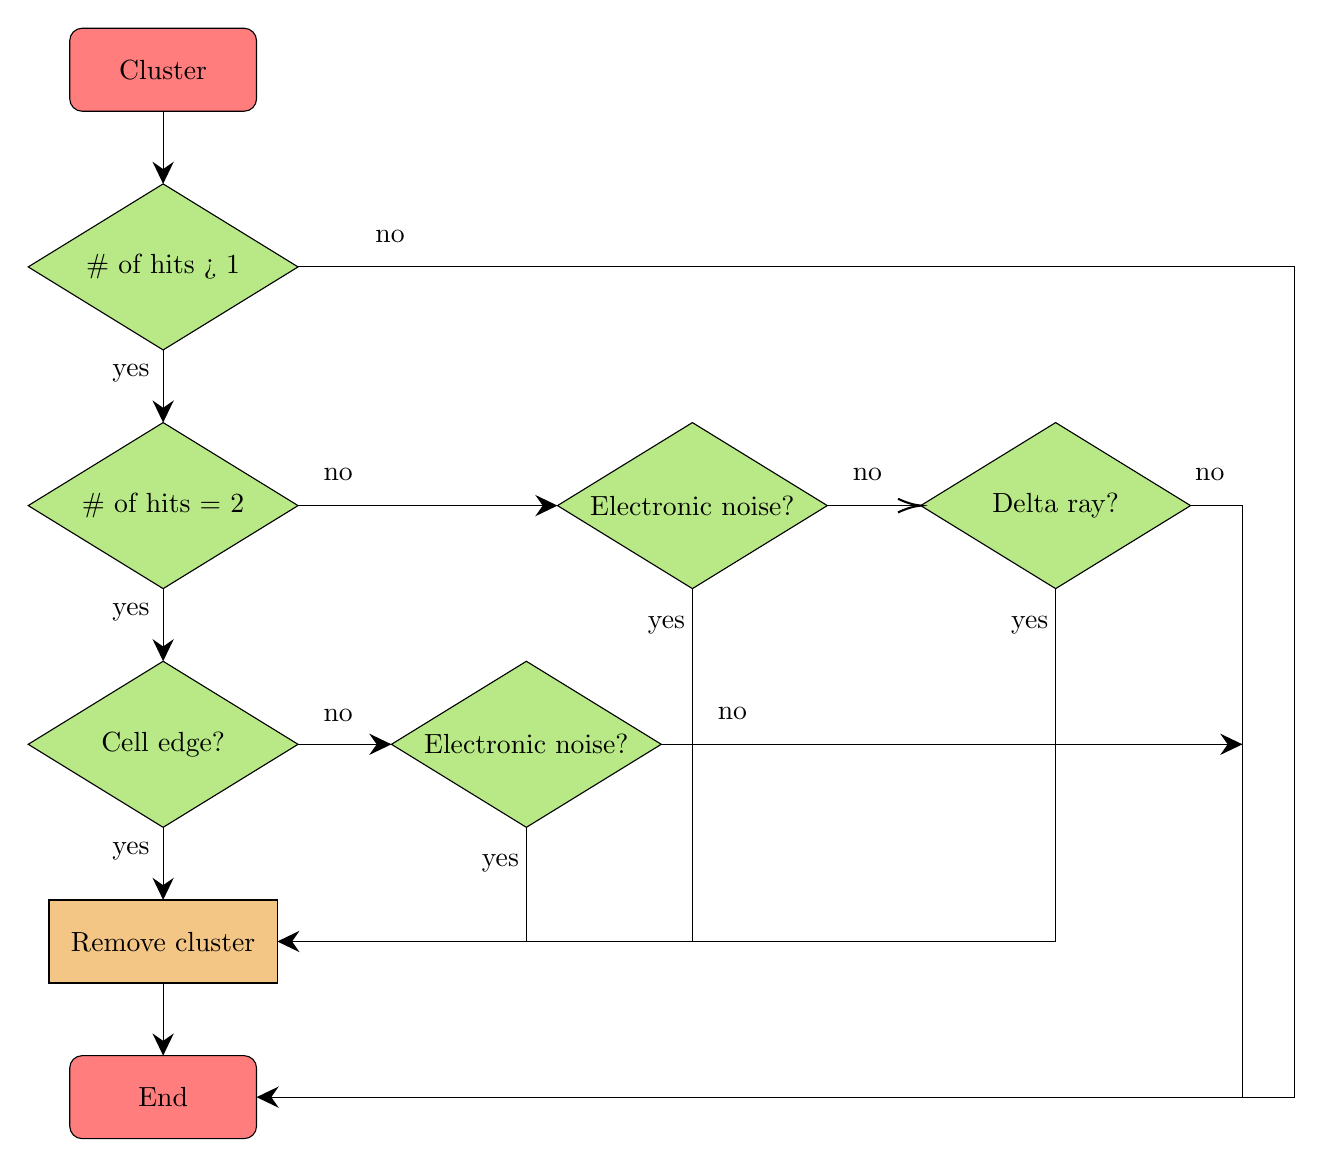
\begin{tikzpicture}[x=0.75pt,y=0.75pt,yscale=-1,xscale=1]
%uncomment if require: \path (0,549); %set diagram left start at 0, and has height of 549

%Rounded Rect [id:dp1662492856064861] 
\draw  [fill={rgb, 255:red, 255; green, 125; blue, 125 }  ,fill opacity=1 ] (20,11) .. controls (20,7.69) and (22.69,5) .. (26,5) -- (104,5) .. controls (107.31,5) and (110,7.69) .. (110,11) -- (110,39) .. controls (110,42.31) and (107.31,45) .. (104,45) -- (26,45) .. controls (22.69,45) and (20,42.31) .. (20,39) -- cycle ;
%Flowchart: Decision [id:dp816640900376574] 
\draw  [fill={rgb, 255:red, 184; green, 233; blue, 134 }  ,fill opacity=1 ] (240,310) -- (305,350) -- (240,390) -- (175,350) -- cycle ;
%Flowchart: Decision [id:dp3056798665151721] 
\draw  [fill={rgb, 255:red, 184; green, 233; blue, 134 }  ,fill opacity=1 ] (320,195) -- (385,235) -- (320,275) -- (255,235) -- cycle ;
%Straight Lines [id:da43332826362990795] 
\draw    (65,45) -- (65,77) ;
\draw [shift={(65,80)}, rotate = 270] [fill={rgb, 255:red, 0; green, 0; blue, 0 }  ][line width=0.08]  [draw opacity=0] (10.72,-5.15) -- (0,0) -- (10.72,5.15) -- (7.12,0) -- cycle    ;
%Straight Lines [id:da1721933893310973] 
\draw    (65,160) -- (65,192) ;
\draw [shift={(65,195)}, rotate = 270] [fill={rgb, 255:red, 0; green, 0; blue, 0 }  ][line width=0.08]  [draw opacity=0] (10.72,-5.15) -- (0,0) -- (10.72,5.15) -- (7.12,0) -- cycle    ;
%Straight Lines [id:da7629068372469668] 
\draw    (130,235) -- (252,235) ;
\draw [shift={(255,235)}, rotate = 180] [fill={rgb, 255:red, 0; green, 0; blue, 0 }  ][line width=0.08]  [draw opacity=0] (10.72,-5.15) -- (0,0) -- (10.72,5.15) -- (7.12,0) -- cycle    ;
%Straight Lines [id:da2682927683523839] 
\draw    (130,350) -- (172,350) ;
\draw [shift={(175,350)}, rotate = 180] [fill={rgb, 255:red, 0; green, 0; blue, 0 }  ][line width=0.08]  [draw opacity=0] (10.72,-5.15) -- (0,0) -- (10.72,5.15) -- (7.12,0) -- cycle    ;
%Shape: Rectangle [id:dp937184065620104] 
\draw  [fill={rgb, 255:red, 244; green, 198; blue, 133 }  ,fill opacity=1 ] (10,425) -- (120,425) -- (120,465) -- (10,465) -- cycle ;
%Straight Lines [id:da7703418793683412] 
\draw    (130,120) -- (610,120) -- (610,520) -- (113,520) ;
\draw [shift={(110,520)}, rotate = 360] [fill={rgb, 255:red, 0; green, 0; blue, 0 }  ][line width=0.08]  [draw opacity=0] (10.72,-5.15) -- (0,0) -- (10.72,5.15) -- (7.12,0) -- cycle    ;
%Straight Lines [id:da9159913508501855] 
\draw    (560,235) -- (585,235) -- (585,520) ;
%Straight Lines [id:da9876271822829807] 
\draw    (305,350) -- (582,350) ;
\draw [shift={(585,350)}, rotate = 180] [fill={rgb, 255:red, 0; green, 0; blue, 0 }  ][line width=0.08]  [draw opacity=0] (10.72,-5.15) -- (0,0) -- (10.72,5.15) -- (7.12,0) -- cycle    ;
%Straight Lines [id:da06393806538831526] 
\draw    (320,275) -- (320,445) -- (123,445) ;
\draw [shift={(120,445)}, rotate = 360] [fill={rgb, 255:red, 0; green, 0; blue, 0 }  ][line width=0.08]  [draw opacity=0] (10.72,-5.15) -- (0,0) -- (10.72,5.15) -- (7.12,0) -- cycle    ;
%Straight Lines [id:da5394607907564043] 
\draw    (240,390) -- (240,445) ;
%Rounded Rect [id:dp009664062523304096] 
\draw  [fill={rgb, 255:red, 255; green, 125; blue, 125 }  ,fill opacity=1 ] (20,506) .. controls (20,502.69) and (22.69,500) .. (26,500) -- (104,500) .. controls (107.31,500) and (110,502.69) .. (110,506) -- (110,534) .. controls (110,537.31) and (107.31,540) .. (104,540) -- (26,540) .. controls (22.69,540) and (20,537.31) .. (20,534) -- cycle ;
%Flowchart: Decision [id:dp9024602763737721] 
\draw  [fill={rgb, 255:red, 184; green, 233; blue, 134 }  ,fill opacity=1 ] (65,80) -- (130,120) -- (65,160) -- (0,120) -- cycle ;
%Flowchart: Decision [id:dp13524885014891452] 
\draw  [fill={rgb, 255:red, 184; green, 233; blue, 134 }  ,fill opacity=1 ] (65,195) -- (130,235) -- (65,275) -- (0,235) -- cycle ;
%Flowchart: Decision [id:dp2973369440123841] 
\draw  [fill={rgb, 255:red, 184; green, 233; blue, 134 }  ,fill opacity=1 ] (65,310) -- (130,350) -- (65,390) -- (0,350) -- cycle ;
%Straight Lines [id:da3005280685773618] 
\draw    (65,275) -- (65,307) ;
\draw [shift={(65,310)}, rotate = 270] [fill={rgb, 255:red, 0; green, 0; blue, 0 }  ][line width=0.08]  [draw opacity=0] (10.72,-5.15) -- (0,0) -- (10.72,5.15) -- (7.12,0) -- cycle    ;
%Straight Lines [id:da23847540301482073] 
\draw    (65,390) -- (65,422) ;
\draw [shift={(65,425)}, rotate = 270] [fill={rgb, 255:red, 0; green, 0; blue, 0 }  ][line width=0.08]  [draw opacity=0] (10.72,-5.15) -- (0,0) -- (10.72,5.15) -- (7.12,0) -- cycle    ;
%Straight Lines [id:da3670573044208534] 
\draw    (65,465) -- (65,497) ;
\draw [shift={(65,500)}, rotate = 270] [fill={rgb, 255:red, 0; green, 0; blue, 0 }  ][line width=0.08]  [draw opacity=0] (10.72,-5.15) -- (0,0) -- (10.72,5.15) -- (7.12,0) -- cycle    ;
%Flowchart: Decision [id:dp8842077208983076] 
\draw  [fill={rgb, 255:red, 184; green, 233; blue, 134 }  ,fill opacity=1 ] (495,195) -- (560,235) -- (495,275) -- (430,235) -- cycle ;
%Straight Lines [id:da6121514959321354] 
\draw    (385,235) -- (428,235) ;
\draw [shift={(430,235)}, rotate = 180] [color={rgb, 255:red, 0; green, 0; blue, 0 }  ][line width=0.75]    (10.93,-3.29) .. controls (6.95,-1.4) and (3.31,-0.3) .. (0,0) .. controls (3.31,0.3) and (6.95,1.4) .. (10.93,3.29)   ;
%Straight Lines [id:da04710382732336604] 
\draw    (495,275) -- (495,445) -- (320,445) ;

% Text Node
\draw (65,25) node   [align=left] {\begin{minipage}[lt]{34.68pt}\setlength\topsep{0pt}
\begin{center}
Cluster
\end{center}

\end{minipage}};
% Text Node
\draw (65,120) node   [align=left] {\begin{minipage}[lt]{60pt}\setlength\topsep{0pt}
\begin{center}
\# of hits > 1
\end{center}

\end{minipage}};
% Text Node
\draw (65,235) node   [align=left] {\begin{minipage}[lt]{60pt}\setlength\topsep{0pt}
\begin{center}
\# of hits = 2
\end{center}

\end{minipage}};
% Text Node
\draw (65,350) node   [align=left] {\begin{minipage}[lt]{49.64pt}\setlength\topsep{0pt}
\begin{center}
Cell edge?
\end{center}

\end{minipage}};
% Text Node
\draw (240,350) node   [align=left] {Electronic noise?};
% Text Node
\draw (320,235) node   [align=left] {Electronic noise?};
% Text Node
\draw (65,445) node   [align=left] {\begin{minipage}[lt]{72.76pt}\setlength\topsep{0pt}
\begin{center}
Remove cluster
\end{center}

\end{minipage}};
% Text Node
\draw (65,520) node   [align=left] {End};
% Text Node
\draw (166,101) node [anchor=north west][inner sep=0.75pt]   [align=left] {no};
% Text Node
\draw (141,216) node [anchor=north west][inner sep=0.75pt]   [align=left] {no};
% Text Node
\draw (141,332) node [anchor=north west][inner sep=0.75pt]   [align=left] {no};
% Text Node
\draw (396,216) node [anchor=north west][inner sep=0.75pt]   [align=left] {no};
% Text Node
\draw (331,331) node [anchor=north west][inner sep=0.75pt]   [align=left] {no};
% Text Node
\draw (36,166) node [anchor=north west][inner sep=0.75pt]   [align=left] {\begin{minipage}[lt]{18.36pt}\setlength\topsep{0pt}
\begin{center}
yes
\end{center}

\end{minipage}};
% Text Node
\draw (36,281) node [anchor=north west][inner sep=0.75pt]   [align=left] {\begin{minipage}[lt]{18.36pt}\setlength\topsep{0pt}
\begin{center}
yes
\end{center}

\end{minipage}};
% Text Node
\draw (36,396) node [anchor=north west][inner sep=0.75pt]   [align=left] {\begin{minipage}[lt]{18.36pt}\setlength\topsep{0pt}
\begin{center}
yes
\end{center}

\end{minipage}};
% Text Node
\draw (214,402) node [anchor=north west][inner sep=0.75pt]   [align=left] {\begin{minipage}[lt]{18.36pt}\setlength\topsep{0pt}
\begin{center}
yes
\end{center}

\end{minipage}};
% Text Node
\draw (294,287) node [anchor=north west][inner sep=0.75pt]   [align=left] {\begin{minipage}[lt]{18.36pt}\setlength\topsep{0pt}
\begin{center}
yes
\end{center}

\end{minipage}};
% Text Node
\draw (495,235) node   [align=left] {Delta ray?};
% Text Node
\draw (469,287) node [anchor=north west][inner sep=0.75pt]   [align=left] {\begin{minipage}[lt]{18.36pt}\setlength\topsep{0pt}
\begin{center}
yes
\end{center}

\end{minipage}};
% Text Node
\draw (561,216) node [anchor=north west][inner sep=0.75pt]   [align=left] {no};


\end{tikzpicture}

	\caption{Flowchart depicting the cluster removal procedure.}
\end{figure}

\paragraph{Trigger Hodoscope masking}
As the hodoscopes have a shorter time resolution compared to the chamber drift time and
the RF bucket periodicity, the hodoscopes are used for triggering. The hodoscope hits
are recorded by both the FPGA trigger modules as well as the TW-TDC. The in-time hodoscope
hits from all 4 stations are combined to form all possible combinations, called road. These
combinations are checked against the active trigger road set used. Only the chamber hits
that fall behind a fired hodoscope paddle, of which is part of a valid trigger road, will be retained.


\subsection{Track Finding}
Following the hit removal stage, the next stage is to find single muon tracks.
The first step in the single track reconstruction is the build tracklets in St.~2 and St.~3.

A tracklet is a small track segment inside each drift chamber. Starting with the $X$ and
$X'$ planes, a hit pairs is formed by locating a hit on each plane within half of a cell spacing.
The position of the a pair is taken as the average of the two hits, and is used to select a window
in the $UU'$ planes to search for corresponding pairs. A window is then selected to locate hit pairs
on the $VV'$ planes. Once the hits are selected, a straight tracklet can be fitted to the hits.
To be considered valid, there must be at least 4 hits, with at least one hit per view. The trackelts
should also be pointing at the target (or beam dump), this is done by requiring the x and y slope to be
less than $(0.15,0.1)$.

Once all tracklets are constructed separately in St.~2 and St.~3. We try to connect a tracklet
in St.~2 with a tracklet in St.~3 to form a partial track. Since there are no magnet between
St.~2 and St.~3, the slope of the tracklets should be similarly. The partial track is then used to
identify hits in the St.~4 proportional tubes for muon identification. The multiple scattering of
muons due to the iron wall between St.~3 and St.~4 is also taken into account.

The St.~2 St.~3 partial track is then projected on to St.~1. The magnetic field of KMag is taken into
account during this step. Since the magnetic field strength is fixed, the sagitta ratio of St.~1 to
St.~2 is approximately a constant and is determined using Monte Carlo simulation. Using this fact,
the search window on St.~1 is constrained by this ratio.

\pdfcomment{kalment filter}

\subsection{Vertex Finding}
Once all the tracks are found in each events, the reconstruction of the dimuon vertex can begin.
For Matrix-1 events, all possible combinations of $\mu^+$ and $\mu^-$ are tested if they can form
a dimuon.

\pdfcomment{kalment filter}

\section{Background Simulation}
\label{sec:mixing}
To obtain the profile of the accidental background, the MATRIX 4 events are used.
MATRIX 4 triggers when there is a single track. 

The accidental background template is created by combining a $\mu^+$ track with
another $\mu^-$ track from a different event. This method is first proposed by 
J.~Dove \cite{dove2020}. 

The MATRIX 4 events are first process by the same track finding procedure as with 
the MATRIX 1 dimuon data. 

To reproduce the MATRIX 1 triggers, the MATRIX 4 tracks are then separated in bins
based on the charge and top/bottom halves of the spectrometer. Since the MATRIX 1
requires the two opposite tracks to be on different halves on the spectrometer,
a positive tracks in the top half would only mixed with a negative tracks in the 
bottom half of the spectrometer, and vice versa. The MATRIX 4 data is also separated
based on the target position. During the mixing procedure, only the tracks from same
target would be analysis together.
The data can also optionally binned in the occupancy to study the intensity dependence
of the accidental background. 

In order to preserve any change in performance in the spectrometer over time, all the
MATRIX 4 tracks in each bin is then sorted in time. Tracks are then mixed in chronological order.
While MATRIX 4 triggers if the trigger system identify only a single tracks, it is also
possible for the reconstruction software to find multiple tracks in the same MATRIX 4 event.
In order to prevent tracks from the same events are mixed, a sliding number $d$ can also be introduced.
With this option enabled, the $i$-th positive track would be mixed with the $i+d$-th negative track.
Typically, a sliding number of one is chosen.


Once the two tracks are selected, the mixed event are ready for vertex finding. As with the 
real data, the dimuon kinematics variables are calculated. The same dimuon selection will
also be applied and can be compared with the real data. Sine the probability of observing a
single track event is much higher than a two track event, the MATRIX 4 trigger is typically
heavily prescaled to preserve DAQ bandwidth. Typically, a prescale of \num{30000} is used during
normal data taking run, meaning only \num{1} in \num{30000} single track event is record.
A minor beneficent is that this method also ensure the result is reproducible.
Therefore, the amount of available MATRIX 4 data for each target can be limited. The mixed events
from different target can also be combined to increase statistics. For this study, the \ce{LH_2}
and \ce{LD_2} mixed events are combined during the mass fitting.

Alternative accidental background generating methods have also been proposed by different group.
One such method is proposed by K. Liu. In this method, MATRIX 1 events are used. In order to 
change of the spectrometer performance over time, two tracks from the same 1 hour run are selected 
randomly. The two tracks are still require to fulfill the opposite charge and top/bottom requirements. 
The two tracks are also required to have similar occupancy, usually within \SI{10}{\percent}.
Because of the use of MATRIX 1 data, the mixed sample has larger statistics. Therefore, when
using MATRIX 1 mixed sample, target specific mixed sample is used.

Both mixing sample is used for the mass fit studies and the difference is quoted as a source systematic
uncertainty.

\section{Dimuon Selection}
The event selection that is used in this study is based on the study by C.~Brown
\cite{chuck-2111} with some modification to increase acceptance at low mass. These cuts
are categorized into different groups and are tabulated in \cref{table:trackCut,table:dimuonCut,table:physCut,table:occCut}.


\begin{table}[ht!]
	\centering
	\caption{Track level cuts.}
	\label{table:trackCut}
	\begin{tabular}{|m{4.5cm}|m{7cm}|m{3cm}|}
		\hline
		Variable                                                                                                                                                                                 & Description                                                                          & Cut                          \\ \hline
		$\chi^2_{\mathrm{target}}$                                                                                                                                                               & $\chi^2$ when tack is   forced to pass through center of target ($z=\SI{-129}{\cm}$) & $< 15$                       \\ \hline
		$pz_1$                                                                                                                                                                                   & z momentum at station 1                                                              & (\SI{9}{\GeV},\SI{75}{\GeV}) \\ \hline
		nHits                                                                                                                                                                                    & total number of hits on wire chambers by each   muon track                           & $> 13$                       \\ \hline
		$x_T^2 +(y_T - \mathrm{beamOffset})^2$                                                                                                                                                   & radial distance of track from   beam line at the center of target                    & $< \SI{320}{\cm\squared}$    \\ \hline
		$x_D^2 +(y_D - \mathrm{beamOffset})^2$                                                                                                                                                   &
		radial distance of track from   beam line at the center of beam dump ($z=\SI{42}{\cm}$)                                                                                                  &
		(\SI{8}{\cm\squared},\SI{1100}{\cm\squared})   \footnotemark[1]                                                                                                                                                                                                                                                \\ \hline
		\begin{tabular}[c]{@{}c@{}}$\chi^2_{\mathrm{target}}<1.5\chi^2_{\mathrm{upstream}}$\\      $\chi^2_{\mathrm{target}}<1.5\chi^2_{\mathrm{dump}}$\end{tabular} &
		$\chi^2$ when tack is   forced to pass through $z=\SI{-490}{\cm}$(upstream), $z=\SI{-129}{\cm}$(traget) and   $z=\SI{42}{\cm}$(dump)                                                     &
		\\ \hline
		$z_0$                                                                                                                                                                                    & z position of track's closest approach to beam   line                                & (\SI{320}{\cm},\SI{-5}{\cm}) \\ \hline
		$\chi^2/(\mathrm{nHits}-5)$                                                                                                                                                              & $\chi^2/\mathrm{ndf}$                                                                & $<12$                        \\ \hline
		$y_1/y_3$                                                                                                                                                                                & y position of track ast St.~1   and St.~3                                            & $<1$                         \\ \hline
		$y_1\times y_3$                                                                                                                                                                          &                                                                                      & $>0$                         \\ \hline
		$| |px_1 - px_3| -0.416|$                                                                                                                                                                & difference in x momentum at St.~1 and St.~3 accounting for the Kmag kick             & $<\SI{0.008}{\GeV}$          \\ \hline
		$|py_1 - py_3|$                                                                                                                                                                          & difference in y momentum at St.~1 and St.~3                                          & $<\SI{0.008}{\GeV}$          \\ \hline
		$|pz_1 - pz_3|$                                                                                                                                                                          & difference in z momentum at St.~1 and St.~3                                          & $<\SI{0.08}{\GeV}$           \\ \hline
		$|py_1 |$                                                                                                                                                                                & absolute value of the y momentum   at St.~1                                          & $>\SI{0.02}{\GeV}$           \\ \hline
	\end{tabular}
\end{table}
\begin{table}[ht!]
	\centering
	\caption{dimuon level cuts.}
	\label{table:dimuonCut}
	\begin{tabular}{|m{4.5cm}|m{7cm}|m{3cm}|}
		\hline
		Variable                                                                                                                          & Description                                                                              & Cut                            \\ \hline
		$|dx|$                                                                                                                            & x position of dimuon vertex                                                              & $<\SI{0.25}{\cm}$              \\ \hline
		$|dy-\mathrm{beamOffset}|$                                                                                                        & y position of dimuon vertex                                                              & $<\SI{0.22}{\cm}$              \\ \hline
		$dz$                                                                                                                              & z position of dimuon vertex                                                              & (\SI{-280}{\cm},\SI{-5}{\cm})  \\ \hline
		$dx^2+(dy-\mathrm{beamOffset})^2$                                                                                                 & radial distance of the dimuon vertex from beam line                                      & $<\SI{0.06}{\cm\squared}$      \\ \hline
		$|dpx|$                                                                                                                           & absolute value of dimuon x   momentum                                                    & $<\SI{1.8}{\GeV}$              \\ \hline
		$|dpy|$                                                                                                                           & absolute value of dimuon y   momentum                                                    & $<\SI{2}{\GeV}$                \\ \hline
		$dpx^2+dpy^2$                                                                                                                     & transverse momentum squared of   dimuon                                                  & $<\SI{5}{\GeV}$                \\ \hline
		dpz                                                                                                                               & dimuon z momentum                                                                        & (\SI{38}{\GeV},\SI{116}{\GeV}) \\ \hline
		$|\mathrm{tackSeparation}|$                                                                                                       & distance in z between points   of  closest approach between $\mu^+$   and $\mu^-$ track  & $<\SI{270}{\cm}$               \\ \hline
		$\chi^2_{\mathrm{dimuon}}$                                                                                                        & $\chi^2$ when both $\mu^+$ and   $\mu^-$ tracks are forced to pass through dimuon vertex & $<18$                          \\ \hline
		$\begin{aligned} |\chi^2_{\mathrm{target}}(\mu^+) &+ \chi^2_{\mathrm{target}}(\mu^-)\\& -\chi^2_{\mathrm{dimuon}}| \end{aligned}$ &                                                                                          & $<2$                           \\ \hline
		$y_3(\mu^+) \times y_3(\mu^-)$                                                                                                    & y position at St.~3 for both tracks                                                      & $<0$                           \\ \hline
		$\mathrm{nHists}(\mu^+)+\mathrm{nHists}(\mu^-)$                                                                                   & sum of the total number if hits on wire chamber by $\mu^+$ and $\mu^-$ track             & $>29$                          \\ \hline
		$\mathrm{nHists}_1(\mu^+)+\mathrm{nHists}_1(\mu^-)$                                                                               & sum of the total number if hits on St.~1 wire chamber by $\mu^+$ and $\mu^-$ track       & $>8$                           \\ \hline
		$|x_1(\mu^+) + x_1(\mu^-)|$                                                                                                       & sum off x position of of tracks   at St.~1                                               & $>\SI{42}{\cm}$                \\ \hline
	\end{tabular}
\end{table}
\begin{table}[h!]
	\centering
	\caption{ physics cuts}
	\label{table:physCut}
	\begin{tabular}{|m{4.5cm}|m{7cm}|m{3cm}|}
		\hline
		Variable              & Description                          & Cut                                                            \\ \hline
		mass                  & dimuon mass                          & (\SI{2}{\GeV},\SI{8.8}{\GeV}) \footnotemark[1]\footnotemark[2] \\ \hline
		$x_F$                 & Feynman $x$                          & (-0.1,0.95)                                                    \\ \hline
		$x_{\mathrm{target}}$ & Bjorken $x$ of target                & (0.005,0.55)  \footnotemark[1]                                 \\ \hline
		$|\cos(\theta)|$      & polar angle in Collins-Soper   frame & $<0.5$                                                         \\ \hline
	\end{tabular}
\end{table}
\begin{table}[h!]
	\centering
	\caption{occupancy cuts}
	\label{table:occCut}
	\begin{tabular}{|m{4.5cm}|m{7cm}|m{3cm}|}
		\hline
		Variable                          & Description                                & Cut      \\ \hline
		D1                                & total hits on St.~1 Chamber                & $<400$   \\ \hline
		D2                                & total hits on St.~2 Chamber                & $<400$   \\ \hline
		D3                                & total hits on St.~3 Chamber                & $<400$   \\ \hline
		$D1+D2+D3$                        & total numbers of hits in all wire Chambers & $<1000$  \\ \hline
		Trigger intensity\footnotemark[3] & numbers of proton in the triggering bucket & $<80000$ \\ \hline
	\end{tabular}
\end{table}

\footnotetext[1]{modified from Ref.~\cite{chuck-2111}}
\footnotetext[2]{The 0.99 scaling factor is applied to MC}
\footnotetext[3]{Not applied to MC or Mix background}
\clearpage
\section{Beam Luminosity Normalization}\pdfmargincomment{might move this section to spectrometer}
\label{sec:beam_norm}
At SeaQuest, there are three beam luminosity related quantities.
During data taking, the proton on target is monitored by two sets of instruments, a secondary
emission monitor located upstream of the SeaQuest experimental hall, and a Cerenkov counter
(as described in \cref{M-subsec:BIM}). The secondary emission monitor provides the integrated
beam intensity for the entire beam spill (labeled as ``G2SEM"). This is sometimes refer to as
``raw proton'' as this quantity does not include any deadtime or inhibit effect.

The Cerenkov counter provides the beam intensity for each RF bucket in relative units.
During normal data taking, the Beam DAQ records three quantities: integrated beam intensity for entire spill
(labeled as ``QIEsum''), integrated beam while inhibit is asserted at trigger logic
(labeled as ``inhibit\_block\_sum'') and integrated intensity during dead time (labeled as
``trigger\_sum\_no\_inhibit''). All these quantities are in relative units.

The number of protons on targets during DAQ live time can be calculated as follows:
\begin{equation}
	\mathrm{live\ proton} = \frac{\mathrm{QIEsum}-\mathrm{inhibit\_block\_sum}-\mathrm{trigger\_sum\_no\_inhibit}}{\mathrm{QIEsum}}\cdot \mathrm{G2SEM}
\end{equation}

The Main DAQ also reads out the beam intensity from Cerenkov counter the of the triggering bucket
and the $\pm16$ RF buckets before and after the trigger (label as ``RF-16" to ``RF+16", with
``RF00'' being the triggering bucket).

The number of proton in the triggering bucket can be calculated as follows:
\begin{equation}
	\mathrm{trigger\ intensity} = \frac{\mathrm{RF00}-\mathrm{pedestal}}{\mathrm{QIEsum}-\mathrm{pedestal}\cdot 588\cdot 369000}\cdot \mathrm{G2SEM}
\end{equation}
The pedestal comes from the dark rate of the detector, and it is obtained from studying the
empty spills. This value can change overtime and is summarize in \cref{tabel:pedestal}.
This number should be subtracted from the bucket specific QIE value, as well as the spill
integrated QIEsum. There are a total of $588\cdot 369000$ buckets per spill, hence the
numerator.

\begin{table}[h!]
	\centering
	\caption{Summary of the QIE pedestal over time\cite{kenichi-9289}.}
	\label{tabel:pedestal}
	\begin{tabular}{|c|c|c|}
		\hline
		Run     & spill range                     & pedestal value \\ \hline
		2-3     &                                 & $34\pm5$       \\ \hline
		5ea-5eb & $[\num{910000},\num{1010000})$  & $33\pm 6$      \\ \hline
		5eb     & $[\num{1010000},\num{1100000})$ & $28\pm 5$      \\ \hline
		6       & $[\num{1200000},\num{1320000})$ & $40\pm 12$     \\ \cline{2-3}
		        & $[\num{1320000},\num{1420000})$ & $30\pm 7$      \\ \hline
	\end{tabular}
\end{table}

\section{Intensity Extrapolation}
\label{sec:extrapolation}
Extracting the Drell-Yan cross section ratio using the intensity extrapolation method
is first studied by J.~Dove \cite{dove2020} and A.~Tadepalli \cite{tadepalli2019},
and it is used in Ref.~\cite{dove2021}.
The assumption behind this method is that the accidental background and physics events
would have different intensity dependence. The number of observed physics
events, in the absent of any spectrometer effects, should be linearly proportional to the beam
intensity. On the contrary, the two muons in the accidental background are typical coming from
two separate interactions, and therefore it is expected proportional to the intensity squared.
By taking the ratio of the $(p+p)$ and $(p+d)$ dimuon event rates,
other rate dependence effect would also be cancel out at zero intensity.

The procedure for this method is summarized here. A mass cut at \SI{4.5}{\GeV} is applied to
remove the charmonium decays, leaving only the Drell-Yan dimuons and the accidental background.
Cuts are also applied to exclude region close to the boundaries of the acceptance.
Then the background originated from the interaction with the instruments is estimated by using
the empty flask data normalized by the integrated beam intensity, and is subtracted from the
$p+p$ and $p+d$ data. Third, the $(p+d)/2(p+p)$ ratios are formed by empty flask subtracted
dimuon data, normalized by the beam intensity. The ratio is calculated as a function of the
instantaneous beam intensity measured by the BIM. The ratio is then fitted with the following function
\begin{equation}
	R_i \left(I\right) = p_{0i} + p_1 I + p_2 I^2,
	\label{eq:common_pol2}
\end{equation}
where the parameter $p_1$ and $p_2$ are common to all bins, and the intercept $p_{0i}$ give
the value of the cross section ratio in each $x_T$ bins. Other fit functions are also used
to studied the fit function dependence.

\pdfcomment{intensity distribution plots, integrated over kinematics}

While this method allows for extractions of the Drell-Yan cross section ratio without relying
heavily on simulation, this method cannot be used in the charmonium studies.
Both Drell-Yan process and charmonium production would have the same linear intensity dependence,
hence this method is not be able to distinguish the different physics proccess, and therefore could
not be use in the charmonium studies. Moreover, only the cross section ratio could be obtained in
this method, as the absolute yield and value of rate dependency correction will be needed in
absolute cross section studies, and cannot be obtained from the intensity extrapolation methods.

\section{Mass Spectrum Fitting}
With the goal of obtaining the absolute yield for different process, the mass spectrum fitting
procedure is developed. This also forms the bases of our recent publication\cite{dove2023}.

The event distribution can be expressed as a linear combination of different components,
namely Drell-Yan, chamrmonium decays, accidental background and background from instruments.
These different contributions would have distinct mass spectra, for example, the $J/\psi$
and $\psi^\prime$ decays would have sharp distributions centered around their masses and
can be easily identified. Therefore, the data can be fitted to varies templates to obtain
the relative contribution from each sources.

\paragraph{Physics sources}
The templates for $J/\psi$, $\psi'$ and Drell-Yan are obtained by analyzing the messy Monte Carlo
simulation (as described in \cref{subsec:messyMC}).

\paragraph{Empty flask subtraction}
The empty flask data is taken by placing just the flask (filled with vacuum) in the path of
the beam. It is used for understanding the background originating from interactions of the beam
with the flask wall, beam dump or various upstream instrumentation. The normalization of the
empty flask contribution is obtained from the ratio of live protons for the liquid target and
empty flask. The empty flask normalization is then kept fixed during the fitting procedure, while
other components are allowed to float.

\paragraph{Accidental/Mixed background correction}
The mixed sample from the MATRIX 4 is typically used. Due to the limited sample size in the raw
MATRIX 4 data, the statistics of the mixed sample is typically limited. For both \ce{LH_2} and 
\ce{LD_2} studies, the mixed sample from both \ce{LH_2} and \ce{LD_2} are combined. Then the sample
template is used for both \ce{LH_2} and \ce{LD_2} analysis. 

Other mixed sample can also be used. This is done to estimate the systematic uncertainty.


\subsection{TFractionFitter}
To account for the statistical uncertainties in both the data and Monte Carlo
simulation, the TFrationFitter algorithm is used in this analysis \cite{barlow1993}.
This is achieved by performing a standard likelihood fit using Poisson statistics,
while the template, generated from MC, are also varied within statistics, leading
to additional contributions to the overall likelihood.

Let there are $m$ sources. The number of MC events in bin $i$ from source $j$
is given by $a_{ji}$. For each source, there is some (unknown) expected distribution
$A_{ji}$. The expected number of events in each bin is given by
\begin{equation}
	f_i = \sum^m_{j=1} p_j A_{ji}.
	\label{eq:TF_f}
\end{equation}
From each $A_{ji}$, the number of Monte Carlo events $a_{ji}$ is obtained.
The total likelihood is the combined probability of the number observed events $\left\{d_i\right\}$
and the number of MC events $\left\{a_{ji}\right\}$
\begin{equation}
	\ln \mathcal{L} = \sum^n_{i=1} d_i \ln f_i -f_i + \sum^n_{i=1} \sum^m_{j=1} a_{ji} \ln A_{ji} - A_{ji}.
	\label{eq:TF_likelihood}
\end{equation}
The estimates for the strength $p_j$ and the expected distribution $A_{ji}$ are
found by maximizing this likelihood. One consequence of this approach is the
$n \cross m$ fit parameters $A_{ji}$. However, the  minimization of these additional
parameters is done analytically ratter than treating them as formal fit parameters.

In the case of weighted MC, \cref{eq:TF_f} is modified into
\begin{equation}
	f_i = \sum^m_{j=1} p_j w_{ji}A_{ji},
\end{equation}
where $w_{ji}$ is the average weight of the MC events in bin $i$ from the source $j$.

\subsection{Tracking Efficiency}
The tracking efficiency is obtained but studying the messy and clean Monte Carlo.
As the detector occupancy increases, the is a higher probability for kTracker to
remove the wrong hit during the EventReducer stage. Therefore, events with higher occupancy
would failed to be reconstructed at a higher rate than low occupancy events. Since the occupancy
is correlated between different tracking stations, we parameterize the tracking efficiency
as a function of one of chambers. In early studies, it is typically parameterized using St.~1
occupancy (D1), however, I chose to use the St.~2 occupancy (D2) in this study. This
is due to the addition of the new chamber at St.~1 in later runs, and using D2 ensures the
extract efficiency can be compared between datasets. The occupancy is defined as the number of
in-time hits in the chamber.

The ratio of reconstructed events of messy over clean MC is plotted in \cref{fig:tracking efficiency}.
\begin{figure}[h!]
	\centering
	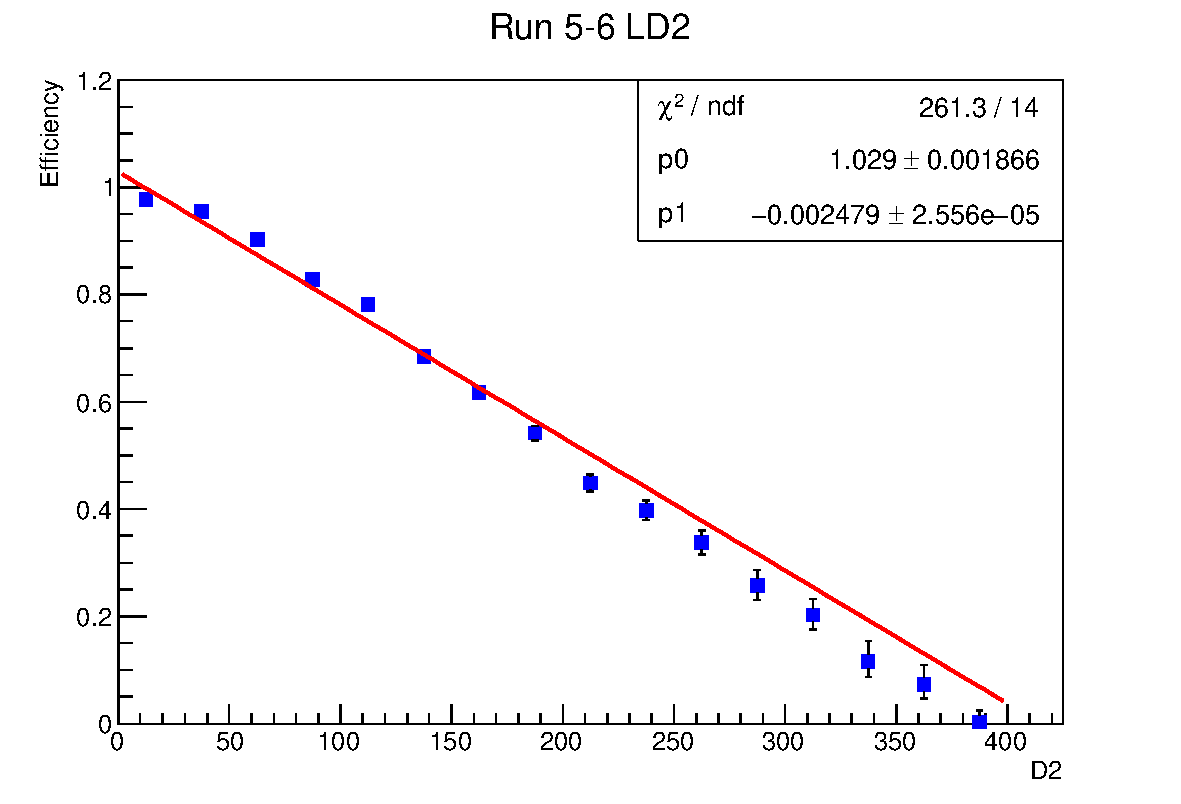
\includegraphics[width=0.5\linewidth]{run5-6_Drell-Yan_LD2}
	\caption{The reconstruction efficiency plotted as a function of station 2 occupancy, calculated using
		Run 5 \ce{LD_2} Drell-Yan MCs.
		The efficiency is calculated by taking the ratio of messy MC events over clean MC events in each
		occupancy bin. Standard cuts were applied to both numerator and denominator
		(except the occupancy cut on clean MC).
	}
	\label{fig:tracking efficiency}
\end{figure}
\pdfcomment{fit to messy/clean}

This tracking efficiency can also depends on the dimuon kinematics. This can be caused
by the noise hits are more localized in some area of the detector, which can mapped to
different kinematic phase space. To study this effect, we repeat the study with different
Monte Carlo, and the extract efficiency is shown in
\pdfcomment{table of efficiency for different target, process and runs}

Once the tracking efficiency obtained from the Monte Carlo, the efficiency correction ($\epsilon_{recon.Eff}$)
is calculated, which is defined as the average of the inverse of tracking efficiency in each
kinematic bin. This correction is calculated separately for each target, as a denser target
will produce more hits in the detector. This is shown in \cref{fig:target_D2}.

\begin{figure}[h!]
	\centering
	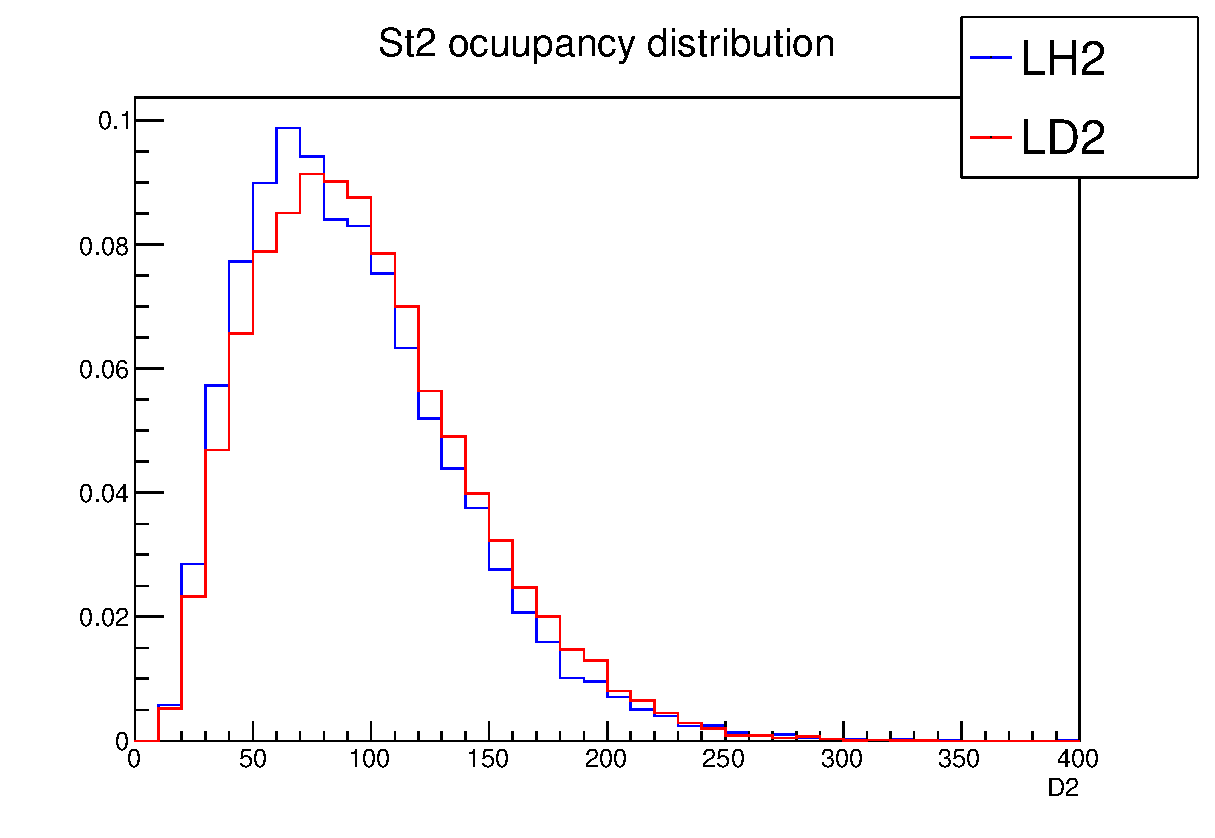
\includegraphics[width=0.5\linewidth]{run5-6_DY_D2}
	\caption{The St.~2 occupancy profile for \ce{LH_2} and \ce{LD_2} for run 5-6 after event selection. Both histogram are normalized to unit area.
	}
	\label{fig:target_D2}
\end{figure}
\pdfcomment{fig:target D2}

\section{Absolute \texorpdfstring{$J/\psi$}{J/psi} Cross Section Extraction}
\subsection{Target Contamination}
For a pure target, the cross section can be obtained from the yield using the following
\begin{equation}
	\sigma = \frac{Y A}{T N_A P X \epsilon},
\end{equation}
where $Y$ is the extracted yield, $A$ is the atomic mass of the target,
$T$ is the thickness of the target, $N_A$ is the Avogadro’s number,
$P$ is the proton on target, $\epsilon$ is the acceptance and efficiency correction,
and $X$ is the beam attenuation factor given by
\begin{equation}
	X=\frac{\lambda}{L\rho} \left[1-\exp\left(-\frac{L\rho}{\lambda}\right)\right],
\end{equation}
where $\lambda$ is the interaction length, $L$ and $\rho$ are the length and density
of the target.

The liquid targets are held in a flask \SI{50.8}{\cm} long and \SI{7.62}{\cm} in diameter
and can contain \SI{2.2}{\l} of liquid. The liquid Hydrogen used is \SI{99.999}{\percent}
pure. On the other hand, the Deuterium used came from two sources:
\begin{itemize}
	\item \SI{95.8\pm0.2}{\percent} pure deuterium that was used for bubble chamber experiments
	      at Fermilab, with contamination in the form of \ce{HD}.
	\item \SI{99.99}{\percent} pure commercial deuterium which is used in later part of the experiment.
\end{itemize}
\begin{table}[h!]
	\centering
	\caption{Summary of \ce{LD_2} contamination, taken from Ref.~\cite{don-4993}}
	\label{table:LD2_contamination}
	\begin{tabular}{|l|ll|l|l|}
		\hline
		Sample no. & \multicolumn{2}{l|}{\ce{D_2} bottle no.} & Sample date & description                                                                                                                          \\ \hline
		1          & \multicolumn{1}{l|}{Fermilab}            & 53          & 4/12/18     & \SI{95.6}{\percent} \ce{D}, \SI{4.4}{\percent} \ce{H}; \SI{92}{\percent}  \ce{D_2}, \SI{8}{\percent} \ce{HD} gases     \\
		2          & \multicolumn{1}{l|}{Fermilab}            & 113         & 4/12/18     & \SI{96}{\percent} \ce{D}, \SI{4}{\percent} \ce{H}; \SI{93}{\percent}  \ce{D_2}, \SI{7}{\percent} \ce{HD} gases         \\
		3          & \multicolumn{1}{l|}{Fermilab}            & 53          & 4/12/18     & just air; gas must have leaked                                                                                         \\
		4          & \multicolumn{1}{l|}{Matheson}            & 127         & 4/12/18     & about half air; remaining \SI{99.1}{\percent} \ce{D}, \SI{0.3}{\percent} \ce{H}                                        \\
		5          & \multicolumn{1}{l|}{Matheson}            & 2           & 4/12/18     & sample for test purposes; not analyzed                                                                                 \\
		6          & \multicolumn{1}{l|}{Matheson}            &             & 7/28/16     & more than half air; remaining \SI{99.3}{\percent} \ce{D}, \SI{0.7}{\percent} \ce{H}                                    \\
		7          & \multicolumn{1}{l|}{Matheson}            &             & 5/28/17     & \SI{99.8}{\percent} \ce{D}, \SI{0.2}{\percent} \ce{H}; \SI{99.6}{\percent}  \ce{D_2}, \SI{0.4}{\percent} \ce{HD} gases \\ \hline
	\end{tabular}
\end{table}
Therefore, care is needed to account for the contribution from the hydrogen contamination in deuterium
target data. The result of the mass spectroscopy of the deuterium gas \cite{don-4993} is
summarized in \cref{table:LD2_contamination}. Based this analysis, it is concluded the Fermilab
deuterium contains \SI{91.6}{\percent} \ce{D_2} and \SI{8.4}{\percent} \ce{HD} by moles. \pdfcomment{need to check this sentence.}

The yield from the contaminated deuterium can be expressed as
\begin{equation}
	Y_{\mathrm{cont.~\ce{LD_2}}} = N_A P_D X_D \epsilon_D \left( T_D^D \sigma_{pd}/A_D + T^D_H \sigma_{pp}/A_H   \right).
\end{equation}
Here $T_D^D$ and $T^D_H$ are the thickness of deuterium and hydrogen in the deuterium target.
The subscript $D$ denote these deuterium target specific quantities.

In order to extract the $T_D^D$ and $T^D_H$ from the mole fraction listed in \cref{table:LD2_contamination},
we first note that the volume of a \ce{HD} molecule is about \num{1.094} times the volume of a \ce{D_2}
molecule. Therefore the effective volume of molecules in the target is
\begin{equation}
	\begin{split}
		V_{\mathrm{eff.}}&=\frac{N_{\ce{HD}} V_{\ce{HD}} + N_{\ce{D_2}} V_{\ce{D_2}}}{N_{\text{tot.}}}\\
		&=V_{D_2} \left[ C \frac{V_{\ce{HD}}}{V_{\ce{D_2}}} + (1-C) \right]\\
		&=V_{D_2} f,
	\end{split}
\end{equation}
where $f=\left[ C \frac{V_{\ce{HD}}}{V_{\ce{D_2}}} + (1-C) \right]$.
The total number of molecules per area is
\begin{equation}
	\begin{split}
		\frac{N_{\mathrm{tot.}}}{\mathrm{Area}} &= \frac{L}{V_{\mathrm{eff.}}}\\
		&= \frac{L}{V_{\ce{D_2}}f}=\frac{L\rho_{\ce{D_2}}}{2A_Df}.
	\end{split}
\end{equation}
The thickness of D (in \unit{\g\per\cm\squared}) in the target cell is
\begin{equation}
	\begin{split}
		T_D^D &= \frac{N_D A_D}{\mathrm{Area}} = A_D\frac{N_{\mathrm{tot.}}}{\mathrm{Area}} \left[ 2(1-C) + C \right]\\
		&=A_D \frac{L\rho_{\ce{D_2}}}{2A_Df}(2-C)\\
		&=\frac{L\rho_{\ce{D_2}}}{f}(1-C/2).
	\end{split}
\end{equation}
The thickness of H (in \unit{\g\per\cm\squared}) in the target cell is
\begin{equation}
	\begin{split}
		T^D_H &= \frac{N_H A_H}{\mathrm{Area}} = A_H\frac{N_{\mathrm{tot.}}}{\mathrm{Area}}C\\
		&=\frac{L\rho_{\ce{D_2}}}{f}\frac{A_H}{A_D}\frac{C}{2}.
	\end{split}
	\label{eq:TDH}
\end{equation}
To determine the density of the deuterium target, the vent pressure is measured and is compared
with NIST database to obtained the expected density for pure deuterium ($\rho_{\ce{D_2}}$) \cite{density-1453}.
For contaminated deuterium, the effective density is
\begin{equation}
	\begin{split}
		\rho_{\mathrm{eff.}} &= \frac{1}{L} (T_D^H + T_D^D)\\
		&=\frac{\rho_{\ce{D_2}}}{f} \left[ \frac{A_H}{A_D}\frac{C}{2}+(1-C/2) \right].
	\end{split}
\end{equation}
and the effective interaction length is
\begin{equation}
	\begin{split}
		\frac{1}{\lambda_{\mathrm{eff.}}} &= \frac{1}{L\rho_{\mathrm{eff.}}} \left[\frac{T_D^H}{\lambda_H} +\frac{T_D^D}{\lambda_D}\right]\\
		&=\left[\frac{A_H}{A_D}\frac{C}{2\lambda_H} + \frac{1-C/2}{\lambda_D}\right]\left( \frac{A_H}{A_D}\frac{C}{2} +(1-C/2)\right)^{-1}.
	\end{split}
\end{equation}

Note that in previous studies and publication, including Ref.~\cite{dove2021}, the ratio of the atomic mass
is missing in \cref{eq:TDH}. This causes a roughly \SI{2}{\percent} difference in the cross section ratio
that will be discussed later.

Thus the deuterium cross section is
\begin{equation}
	\sigma_{pd} = \frac{Y_{\ce{LD_2}} A_D}{T_D^D N_A P_D X_{\mathrm{eff.}} \epsilon_D} - \frac{T^D_H}{T_D^D} \frac{A_D}{A_H} \sigma_{pp},
\end{equation}
where
\begin{equation}
	\sigma_{pp} = \frac{Y_{\ce{LH_2}} A_H}{T_H^H N_A P_D X_{H} \epsilon_H}.
\end{equation}
And the cross section ratio is given by
\begin{equation}
	\frac{\sigma_{pd}}{2\sigma_{pp}} = \frac{Y_{\ce{LD_2}}}{2Y_{\ce{LH_2}}}\frac{A_D}{A_H}\frac{T_H^H P_H X_{H} \epsilon_H}{T_D^D P_D X_{\mathrm{eff.}} \epsilon_D} - \frac{T^D_H}{2T_D^D} \frac{A_D}{A_H}.
\end{equation}

The switch to commercial pure deuterium gas happened during Roadset 67 data taking. Therefore,
an average contamination, weighted by the proton on target, is used for the entire dataset.
The average contamination for entire roadset 57 -70 data is determined to be $C=\SI{5.95}{\percent}$
Therefore the effective values for target contamination for this dataset are
\begin{equation}
	\begin{split}
		T_D^H &= \SI{0.1230}{\g\per\cm\squared}, \\
		T_D^D &= \SI{8.009}{\g\per\cm\squared},\\
		\rho_{\mathrm{eff.}} & = \SI{0.1601}{\g\per\cm\squared},\\
		\lambda_{\mathrm{eff.}} &= \SI{71.39}{\g\per\cm\squared},\\
		\lambda_{\mathrm{eff.}}/\rho_{\mathrm{eff.}} &= \SI{446.0}{\cm},\\
		X_{\mathrm{eff.}} &= 0.9451.
	\end{split}
\end{equation}
And since there is no contamination in the \ce{LH_2} target
\begin{equation}
	\begin{split}
		\rho_{H_2} &= \SI{0.0708}{\g\per\cm\cubed},\\
		T_H^H &= L\rho_{\ce{H_2}} = \SI{3.597}{\g\per\cm\squared},\\
		\lambda_H/\rho_{\ce{H_2}} &= \SI{734.5}{\cm},\\
		X_H &=0.9662.
	\end{split}
\end{equation}


\subsection{Acceptance Calculation}
The acceptance is obtained by comparing the clean Monte Carlo with thrown distribution,
and is defined as follows
\begin{equation}
	\epsilon_{acc.}\left(\Omega\right)=\mathrm{Acceptance}\left(\Omega\right)= \frac{N_{accept}\left(\Omega\right)}{N_{thrown}\left(\Omega\right)},
\end{equation}
where $N_{accept}\left(\Omega\right)$ is the number of accepted events in a given kinematic bin $\Omega$
by analyzing the clean Monte Carlo after passing the analysis procedure as the data, while $N_{thrown}$ is
the total number of generated Monte Carlo events in the same kinematic bin.

The accepted histogram in the numerator is filled using the reconstructed kinematic, whereas
the thrown histogram in the denominator is filled using the thrown kinematic.

Since our histogram are weighted histogram, the uncertainty is calculated using the following
\pdfcomment{verify the uncertainty calculation here}

\section{Comparison of data and Monte Carlo}

\subsection{\texorpdfstring{$P_T$}{P\_T} distribution}



\section{Systematic uncertainties}
For the Drell-Yan cross section ratios studies, the intensity extrapolation method and mass fit
method involve different assumption and therefore different sources of systematic uncertainties.
\paragraph{Proton beam normalization}
The beam normalization uncertainty is present in all studies presented here.
As described in \cref{sec:beam_norm}, the number of protons are measured by the BIM, which is
calibrated against a SEM monitor. The SEM monitor is further calibrated by studying the activation of
an irradiated high purity copper foil. A copper foil is placed in the beam line near the monitor,
causing the production of \ce{^{24}Na}. The \ce{^{24}Na} then decay into \ce{^{24}Mg} through $\beta$
decay. The number of  \ce{^{24}Na} nuclei is deduced by counting the number \SI{1369}{\keV} photons
produced. Using the \SI{3.56}{\milli\barn} production cross section for \ce{^{24}Na} in natural
copper  by \SI{120}{\GeV} protons, the number of incident protons can be deduced. The estimated
random uncertainty in the counting and extraction of \SI{1369}{\keV} peak is $\sim 1-2\%$.
An additional \SI{8}{\percent} systematic uncertainty in the production cross section of \ce{^{24}Na}
is also included \cite{docdb-457,docdb-7708}.
A total of \SI{10}{\percent} beam normalization uncertainty is assigned to absolute cross
section studies, whereas a \SI{2}{\percent} relative normalization uncertainty is assigned to ratios between
targets. This \SI{2}{\percent} relative normalization uncertainty is also included in the empty flask
subtraction.

\paragraph{Choice of fit function}
This is specific to the cross section ratio studies using intensity extrapolation method.
To estimate the effect of the choice of fit function, different fit functions were examined.
For example, we can allow the $p_1$ and $p_2$ parameters in \cref{eq:common_pol2} to have kinematic
dependence
\begin{equation}
	R_i \left(I\right) = p_{0i} + \left[p_{10}+p_{11}x_i\right] I + \left[p_{20}+p_{21}x_i\right] I^2,
\end{equation}
where $x_i$ is the kinematic average in each bin. The difference between the fit functions are used
as the systematic uncertainty.

\paragraph{Mixed background}
This is specific to studies using mass fit method. Different mixing methods have been proposed in SeaQuest.
The mixed sample from the two methods described in \cref{sec:mixing} are studied. The difference between 
the two analysis in included in the systematic uncertainty.

\paragraph{Acceptance simulation}
This is a major systematics in the absolute cross section studies, particularly when using
Run 2-3 data.
During Run 2-3, multiple trigger road sets were used. However, due to the limited statistics in each
data taking period, it is not possible to analysis each subset separately. Therefore these datasets
are combined into one. While the difference in trigger road set have little effect on the acceptance
for the high mass Drell-Yan dimuon \cite{jdove-8168}, the impact on the $J/\psi$ acceptance is much
larger \cite{chleung-9643}.

During later runs, only one trigger road set (roadset 78) was used, hence this is no
longer an issue.



\section{Drell-Yan NLO calculation}
The next-to-leading order (NLO) calculation is done using a parton level Monte
Carlo program written by the INFN group\cite{catani2009,catani2007}. This program
is originally written to compute written to compute cross-section for vector boson
production from $p+p$ and $p+\bar{p}$ collisions. It was later modified, in
collaboration with Wen-Chen Chang and Shivangi Prasad, to perform $p+n$ calculation
by utilizing isospin symmetry. The $p+d$ interaction can be computed by summing up
the $p+p$ and $p+n$ calculation, assuming no nuclear corrections. For heavier nuclear
targets, nuclear PDFs can also be used.

\pdfmargincomment{Error calculations}
The PDF sets used in this study are CT18\cite{hou2019} and NNPDF4.0\cite{ball2021}.
And they are accessed through the LHAPDF library\cite{buckley2015}. It should be noted
that the CT18 PDF set is published before the SeaQuest result, whereas NNPDF4.0
incorporate the SeaQuest measurements\cite{dove2021} in the global fit.

The uncertainty band for calculations using CT18 PDFs are calculated using the hessian methods.
Given a central PDF member $S_0$ and $2N_{\mathrm{par}}$ eigenvector PDF member $S^\pm_i$ ($i=1,\dots,N_{\mathrm{par}}$),
where $N_{\mathrm{par}}$ is the number of parameters. The central value $F_0$ and the uncertainty $\sigma^\pm_F$
on a PDF-dependent quantity are given by:
\begin{equation}
	\begin{split}
		F_0 &= F(S_0),\quad F_i^\pm=F(S_i^\pm) \\
		\sigma^+_F &= \sqrt{\sum_{i=1}^{N_{\mathrm{par}}} \left[\max\left(F_i^+ - F_0, F_0 - F^-_i,0\right)\right]^2 }\\
		\sigma^-_F &= \sqrt{\sum_{i=1}^{N_{\mathrm{par}}} \left[\max\left(F_0 - F^+_i, F_i^- - F_0,0\right)\right]^2 }
	\end{split}
\end{equation}

Whereas the uncertainty for NNPDF4.0 is calculated using the replicas method. Given $N_{\mathrm{rep}}$ replica
PDF members $S^k$, the central value and the uncertainty is given by the mean and standard distribution
\begin{equation}
	\begin{split}
		F_0&=\expval{F}=\frac{1}{N_{\mathrm{rep}}}\sum_{i=1}^{N_{\mathrm{rep}}}F\left(S^k\right)\\
		\sigma_F&= \sqrt{\frac{1}{N_{\mathrm{rep}}-1}\sum_{i=1}^{N_{\mathrm{rep}}}\left[F\left(S^k\right)-F_0\right]^2}
	\end{split}
\end{equation}

It should also be noted that CT18 reports the \SI{90}{\percent} confidence level by default, whereas NNPDF4.0
would report the \SI{68}{\percent} confidence level.

\ifSubfilesClassLoaded{ \printbibliography[heading=bibintoc,title={References}]}{}
\end{document}
